\documentclass[conference]{IEEEtran}
\IEEEoverridecommandlockouts
% The preceding line is only needed to identify funding in the first footnote. If that is unneeded, please comment it out.
\usepackage{cite}
\usepackage{float}
\usepackage{amsmath,amssymb,amsfonts}
\usepackage{graphicx}
\usepackage{textcomp}
\usepackage{xcolor}
\def\BibTeX{{\rm B\kern-.05em{\sc i\kern-.025em b}\kern-.08em
    T\kern-.1667em\lower.7ex\hbox{E}\kern-.125emX}}
\begin{document}

\title{CENG435 TERM PROJECT PART-2 \\ STUDY REPORT \\
{\footnotesize}
\thanks{}
}

\author{\IEEEauthorblockN{ Yavuz Selim YESILYURT}
\IEEEauthorblockA{\textit{2259166} \\
\textit{Group-68}
}
\and
\IEEEauthorblockN{ Gokhan SAN}
\IEEEauthorblockA{\textit{2171916} \\
\textit{Group-68}
}
}

\maketitle

\section{Design and Implementation Part}
\subsection{Project Overview}
The goal of the project is to design and implement a network which consists of a source node, a broker, two routers and a destination node. In this second part, on top of everything that is implemented in part-1, an implementation of multihomed and pipelined RDT between broker and destination has been implemented. Between nodes source and broker, again, TCP (Transmission Control Protocol) is employed. After file is transferred to broker correctly with TCP channel, broker packetizes these byte streams as packets and sends them to the destination (over routers which are configured to forward IPV4 packets between broker and destination) with proper headers over UDP (User Datagram Protocol). RDT between broker and destination is implemented similar to Go-Back-N; meaning, reliability of UDP channel is handled with one timer in broker, checksums of each individual packet, feedback packets from destination, continious timeout interval update in broker and reordering of data packets in destination. Further details about our RDT protocol implementation are discussed in \textit{Design Approach} and \textit{Implementation Approach} parts below. \\

On this constructed network we carry out three experiments for each of three figures regarding Packet Loss Percentage vs File Transfer Time, Corruption percentage vs File Transfer Time and Reordering percentage vs File Transfer Time, respectively. In each of these three figures results are gathered based on 3 different scenarios, basically 3 different experiments. Each of the experiments (in total of 9 experiments) is carried out with many sample executions. The findings about these experiments are plotted to their corresponding graphs with a 95\% confidence interval and with a margin of error less than 2.5\%. Further details about the experiments are discussed in \textit{Experimental Results} part below. \\

For this part, we sit together and designed our architecture. We bumped into several problems and came up with several solutions and ideas. Therefore design of the architecture and solutions for router configurations, experiments and construction of report were collaborative. Afterwards we divided the workload between us as partners. Yavuz Selim was responsible for implementations of broker and destination nodes, commands for synchronizing nodes, configurations and verifications of the router nodes. He was also responsible for making the experiments for the third figure (reordered packets). Gokhan was responsible for implementation of source node, addition/deletion and showing of the network traffic control commands and he was also responsible for making the experiments for the first and the second figures(lost and corrupt packets). README and photos was created by Yavuz Selim and code for plotting the graph and graphs themselves were created by Gokhan. For report, each member was responsible for the parts that is related with his workload. Throughout the whole phase workload, we were synchronized with each other and we were up-to-date with each others work.

\subsection{Design Approach}
A file of size 5MB was needed to be transferred from source to destination reliably and in correct order. Since, earlier in part-1, between source and broker nodes TCP was employed there was no need for any further implementation for reliability of that channel. But since rest of the network was using UDP and its unreliable, mechanisms for reliability on broker and destination nodes was needed to be implemented. \\

Source node sends whole file to broker as byte streams with TCP. But since a file checksum for checking its integrity and correctness and also a starting time for file sending process needed in destination, source sends these information as headers in the very first packet to broker. After file data is transferred to broker correctly source terminates and broker starts breaking data to 900 byte chunks and sends them to destination with proper headers according to constraints similar to Go-Back-N. \\

On broker side; it has a sequence number for tracking the data packets, a buffer for keeping the data to send, base for keeping the base index of current window, a window size (which is set to 20) for sending data packets within the bounds of window, a timeout interval for setting the timeout value for timer. Initially base and sequence number are set to 0 and timeout interval is set to 0.5 second. Timeout interval will be updated per incoming feedback packet. \\

As broker sends packets to destination it packetizes them with a sequence number and current time information (for calculation of sample RTT on incoming ACK packets) and then calculates checksum of the packet for integrity calculation in destination and adds that checksum into packet header, then sends to destination's first (router 1) interface if the sequence number of packet is even, otherwise it sends to destination's second (router 2) interface. Note that packet length has become 32 + 8 + 4 + 900 = 944 bytes (With Ethernet, IP and UDP headers it is approximately 986 bytes). Broker is designed as capable of sending packets as far as sequence number is within the bounds of current window size (if sequence number $<$ base + window size it can send the packet to destination), otherwise it waits for base to slide. Base slides based on ACK packets that comes from destination. In addition, if base equals to sequence number while sending packets, it starts the timer. Finally it increments the sequence number as it sends data packet to destination successfully. \\

As broker sends data to destination, it also listens (from 2 interfaces) for incoming ACK packets from destination. Whenever an ACK packet comes, it first extracts checksum from the packet and then it calculates the checksum of the remaining part of the packet and compares the extracted one and calculated one, in this manner it checks the integrity of the incoming ACK packets. If packet is not corrupt and "Sequence Number of ACK packet + 1" is greater than the current base, it slides base "Sequence Number of ACK packet + 1" many, then it chekcs the sequence number and base, it they are equal, it stops timer, otherwise it first extracts time information (which is stashed into packet when sending it to destination) from ACK packet and calculates "sampleRTT" value from it. Then as in TCP it updates timeout value according to: \\

\begin{center}
\text{estimatedRTT}= (0.875 * \text{estimatedRTT}) + (0.125 * \text{sampleRTT}) \\
\text{devRTT} = (0.75 * \text{devRTT}) + (0.75 * $abs$(\text{sampleRTT} - \text{estimatedRTT})) \\
\text{Timeout Interval} = \text{estimatedRTT} + (4 * \text{devRTT}) \\
\end{center}

Afterwards it starts the timer again with the updated "Timeout Interval" value. If at any point of execution (sending and receiving packets) timer expires; broker gets interrupted and first starts the timer again with current Timeout Interval value and starts sending all the UnAcknowledged packets (from window's base to current sequence number) back to destination consecutively. \\

After all the data is sent to destination correctly (means all the data packets is acknowledged back from destination) it waits a bit for network and destination to get ready again and finally sends the file checksum and file sending process's start time which it received from source at the very first packet that is received from source, to destination. \\

On destination side; it has a expected sequence number which is set to 0 initially and  two data containers for accumulating the incoming correct data. It listens from 2 interfaces (as was in part-1) for incoming packets and as soon as it receives a data packet it extracts the checksum part from it (as done in broker receiving side), then it calculates the checksum of the remaining part of the packet and compares the extracted one and calculated one, in this manner it checks the integrity of the incoming data packets. Afterwards it extracts sequence number and time information from the packet, and if sequence number of the packet equals to the expected sequence number in destination then destination creates an ACK packet with the expected sequence number and time information which is extracted from data packet. Afterwards it calculates checksum of the packet for integrity calculation in broker's receiving side and adds that checksum into feedback packet's header, then sends this packet to broker's first (router 1) interface if expected sequence number is even, otherwise it sends the packet to broker's second (router 2) interface. Note that feedback packet length has become 32 + 8 + 4 + 3 = 47 bytes (3 bytes for "ACK", and with Ethernet, IP and UDP headers it is approximately 89 bytes). Finally it appends the data with its sequence number to data container and increments the expected sequence number. \\

After all the data is received in destination correctly destination first combines its data container then it listens broker to send file checksum and file sending process's start time, as soon as it receives the related data packet, it extracts the file checksum and time information from it. Afterwards it sorts its data container according to their sequence numbers and stores the data into a file which it reads afterwards and calculates its checksum and compares with file checksum which is extracted earlier on the last packet. Then destination reports whether data is transferred correctly or not according to checksum comparison. \\

For routers; they are basically just configured \& used for forwarding incoming packets to next hop, none implementation of reliability has been done on these nodes. \\

In summary, reliability is provided when lost packets, corrupt packets and change of order in packets are handled. With a similar design to Go-Back-N protocol, in our RDT Protocol, these three attributes are handled properly in broker and destination nodes. In addition multihoming is employed in both broker and destination, also pipelining is employed in broker. \\

Starting from the last item, broker sends data pipelined, with a similar design to Go-Back-N. It maintains a base for keeping the start of the window, a window size for keeping a size for window and a buffer for keeping data to send. It is capable of sending "windowSize" many data packets without receiving an ACK packet for "Current Sequence Number - windowSize"$th$ (Base$th$) packet. If UnAcknowledged packet count equals to windowSize, then broker waits for packets from the beginning of the window to get acknowledged, as soon as base slides (meaning some packets from the beginning of the window gets acknowledged) broker slides its window and sends next data packet. \\

Multihoming is achieved in both broker and destination by sending packets from both interfaces according to packets' sequence numbers. While sending packet, both nodes check for the even/odd situation of the sequence number of the packet to be sent and sends packet to other side from proper interface (from proper router). With this manner half of the packets are sent from one link and the other half is sent from other link, so both links of network is utilized, sharing the workload of sending packets. \\

To handle lost packets, broker maintains a timer for the first UnAcknowledged data packet in current window, in which if expires interrupts normal execution, restarts timer and establishes a fast retransmission system. Timer does not expire as soon as acknowledgement packet of a data packet arrives within the timeout boundaries. So until broker receives a feedback packet for the first UnAcknowledged data packet it retransmits the all the data packets in current window back (when timeout expires). In this manner, all sent data packets are guaranteed to be acknowledged by destination as "Received correctly". In addition, for timeout intervals (as explained above) TCP's calculation method is employed. Broker keeps sending time information together with data packets to destination and it gets them back with the ACK packets from destination, with this way it calculates the sampleRTT and updates estimatedRTT, devRTT and Timeout Interval values continiously. \\ 

To handle corrupt packets, while sending; both broker and destination calculates checksum of the packet to be sent and adds that to header of the packet. While receiving; both broker and destination first extracts the checksum field from the packet and calculates the checksum of the remaining part of the packet, then compares the two values, if, in both nodes, a packet checksum does not match on receiving side, that side just does nothing, since that packet's timer in broker is expected to timeout without a correct feedback packet, that side simply reports that packet is corrupt. Since when timeout happens in broker it just retransmits the related data packet (plus window size many packets) again with proper checksums, in this manner, when a packet gets corrupt it is guaranteed to retransmitted back. In addition since source sends file checksum to broker at the beginning of the communication and broker sends it to destination at the end of the communication, destination gets file checksum at the end and it compares it with the calculated checkum of the output file. It reports whether the file is transmitted correctly or not at the end.\\ 

To handle change of order in packets, since reordering of packets may change the acknowledgement order of the data packets, reordered data packets are treated as lost and timer for that packet gets triggered. So, basically, same semantics as in the handling of the lost packets and corrupt packets is employed, namely, if retransmission gets triggered by any of the packet's timer, then that packet gets resent by the broker. In addition, to ensure that data is in correct order in the output file as in the input file, destination keeps data in container with their sequence number (as was in part-1) and before it writes the data to an output file, it sort the data according their sequence numbers. In this manner, order of data packets in destination is guaranteed to be kept same. 

\subsection{Implementation Approach}
The implementation process started by us choosing Python language to write a single script for each node. We decided to embed required information to the packets as character bytes since our data from the file were also in the same form and they would be easy to handle. \\

Then we created our slices on GENI platform by using given tutorials and XML file that defines our topology with assigned manual IP adresses. \\

We started the implementation of nodes from Source node. We created an IPV4 TCP socket to connect to the broker's ready-to-accept TCP socket. Then to calculate md5sum of the file we opened and read from input file. Then we opened the input file again to read and send this time. Afterwards source node was to read 500KB from input file and send that stream to broker. But since the file transmission time is measured between source node and destination and file's integrity is checked at the end on the destination node, we added starting time information and file checksum to the very first packet that is to be sent to broker. Since each device has one or two IP adress to store, we didn't choose to create an IP table for routing but we embedded static IP addresses which are needed to communicate for each node to the script as global variables and named them accordingly. After sending the whole data as 500KB chunks source terminates. \\

Then we implemented the script for the Broker node. The broker node gets the TCP streams, packetizes them and converts them to UDP datagrams to send destination. But since in this part of the term project broker needs to handle communication between destination in reliably, we implemented main structures of RDT protocol here. First thing to do was creating one listening TCP socket (from Source), two listening UDP sockets for 2 interfaces to routers and two outgoing UDP sockets to send the data to destination. For sender UDP sockets, IP addresses and pre-reserved ports of interfaces of destination, which are static, are given to them. For listening sockets, we changed the socket flag to prevent execution from being port-blocked by the operating system for security reasons and we binded them to the proper listen addresses from interfaces (for TCP listening socket, we also set it to listen for incoming messages). We implemented first action of broker such that, it first gets first data packet from 0source and extracts file md5sum and time start information from it, after storing them it iteratively gets whole input file and stores them into a container. After getting whole data file it divides the data(5MB) into 900 byte chunks and stores them into a container named "buff". With this way, a list with 5556 many 900 bytes packets gets created. Afterwards sequence number and base are initialized to 0 and window size is initialized to 20. Timeout interval and estimatedRTT both initialized to 0.5 and devRTT is initialized to 0. Then "Locks" for base, timer and timeout interval variables is defined to ensure that no race condition happens when threads sharing a common data. Also a "Condition" variable is defined to use whenever sender needs to wait for base to slide. Since broker needs to be implemented such that it both sends and listen for incoming data and needs to retransmit data when timer expires, we defined three functions to handle these cases. \\

Sending function is implemented to packetize and send data packets multihomed (meaning it sends the data from both interfaces) and pipelined (meaning whenever there is a gap on window it sends the next packet with sequence number from buffer). Function basically sends the data in buffer in a loop and in each iteration of the loop it checks whether the current sequence number is smaller than base + window size (if there is available space in window), if there is it gets new 900 byte chunk from buffer and checks whether the sequence number is even or odd; if it is even it packs current time information(8 bytes) and sequence number(4 bytes) as header and then calculates the md5sum(32 bytes) of the packet with adding it to the beginning of the data packet, afterwards it sends the packet to destination's first (router1) interface, if sequence number is odd it creates the packet same and sends the packet to destination's second (router2) interface. If there is not available space in window, sender function just waits for base to slide using "baseCond" Condition variable. In addition, after each loop sender waits exactly "0.01" seconds for network and routers to get ready again (since they could not reach the speed of broker). Throughout the function, whenever an access to global-shared variables(base, timer, sequence number) happens its defined Lock is used. \\

Receiving function listens from its interface-dedicated UDP listening socket. Whenever it receives a feedback packet from destination it immediately extracts the checksum field of the packet and calculates the md5sum of the remaining part of the packet. Then it checks whether the cheksums match, if they match it extracts time information and sequence number from feedback packet and slides base "sequence number of packet + 1" many if base is smaller than the "sequence number of packet + 1" value. Upon sliding the base, it notifies the waiting sender thread (if waits) then checks if base equals to current sequence number, if it is, then it stops the timer, else, it first calculates the "sampleRTT" from time information extracted from packet and calculates new Timeout Interval value with a function which does exactly the same calculation of timeout value(timeout value calculation of TCP) which is discussed above. Then it restarts the timer with newly updated value. Throughout the function, whenever an access to global-shared variables(base, timer, sequence number) happens its defined Lock is used. \\

Retransmission function is called by the timer if timeout is reached. It basically restarts the timer with the current timeout value (as in TCP) and starts retransmitting all UnAcknowledged data packets(from base to seqnum) back to destination in a for loop. While retransmitting, as in normal sender function, it checks the even/odd situation of sequence number of packet and sends to destination from proper interface and data packet is packed as the same (first time and sequence number is packed then checksum is calculated and then it is added to the packet). Throughout the function, whenever an access to global-shared variables(base, timer, sequence number) happens its defined Lock is used. \\

For usage of these functions in harmony, first a thread for timer is initialized with initial timeout interval value and set to call retransmission function whenever timer expires. Then a listener thread with first listen interface UDP socket and a listener thread with second listen interface UDP socket are sent to receiving function and started. In main execution, sending function is called. After all the sending job is completed, main execution implicitly waits for threads to finish their jobs. After they finish, after a while of 2 seconds, broker sends file md5checksum, which is extracted from first source packet, and file sending process start time to destination. After that broker terminates. \\

Later, our goal was to configure routers so that they forward our packets between broker and destination. For this, using "ip route" command we added ways(links to corresponding routers) for subnets of other side's(for broker, destination; for destination, broker) interfaces. And then within the routers, we changed system configuration to make it forward incoming IPV4 packets. After doing this we verified its activity with "ping" and traceroute commands from both broker and destination nodes. \\

Destination implementation required two listening UDP sockets to listen indefinetely and send feedback packets back to broker, since there are two routers forwarding packets to the destination. Thus, to achieve this goal, we created a multithreaded mechanism in here too. For keeping track of the incoming data packet's sequence numbers, a variable for expected sequence number is first initialized as 0 and a Lock for it defined(since its a common shared variable among threads). Then, in a generic handler function, firstly, they listen for incoming packets over their interface-dedicated listening UDP sockets. Whenever they get a data packet they immediately extract md5sum from checksum field of the packet then calculate the checksum of the remaining part and compare these values. If values match, time information and sequence number is extracted from data packet. A feedback packet consists of extracted time information and expected sequence number is packed with an "ACK" message, then an md5sum calculation for this packet is generated and packed to the beginning of the packet. Then it is sent to broker with proper interface(since the threads listen from a dedicated interface, they also send their packets from this dedicated interface, so the workload of sending feedback packets is also divided into 2). Then expected sequence number is incremented by one and data is appended to data container with its sequence number. Throughout the function, whenever an access to expected sequence number happens its defined Lock is used. \\

After sending process is complete, main execution returns and waits implicitly for other thread to finish its job. Then it waits for last data packet from broker, which contains file checksum and beginning of the file sending time. As soon as it receives the packet  it extracts the md5sum of file and start time. Quickly, it calculates and reports the file sending time and then sorts packets on data container according to their sequence numbers. Afterwards, it writes sorted data on container to an output file which it opens again after writing for calculation of md5sum. After comparing the calculated and received checksum values, it reports whether the input file is transmitted correctly or not. \\

Figure 1 shows a screenshot of an example start-up vision for the process, Figure 2 shows a screenshot of an example halfway execution vision of the process and Figure 3 shows a screenshot of an example finishing vision of the process. \\

\begin{figure}[H]
    \centering
    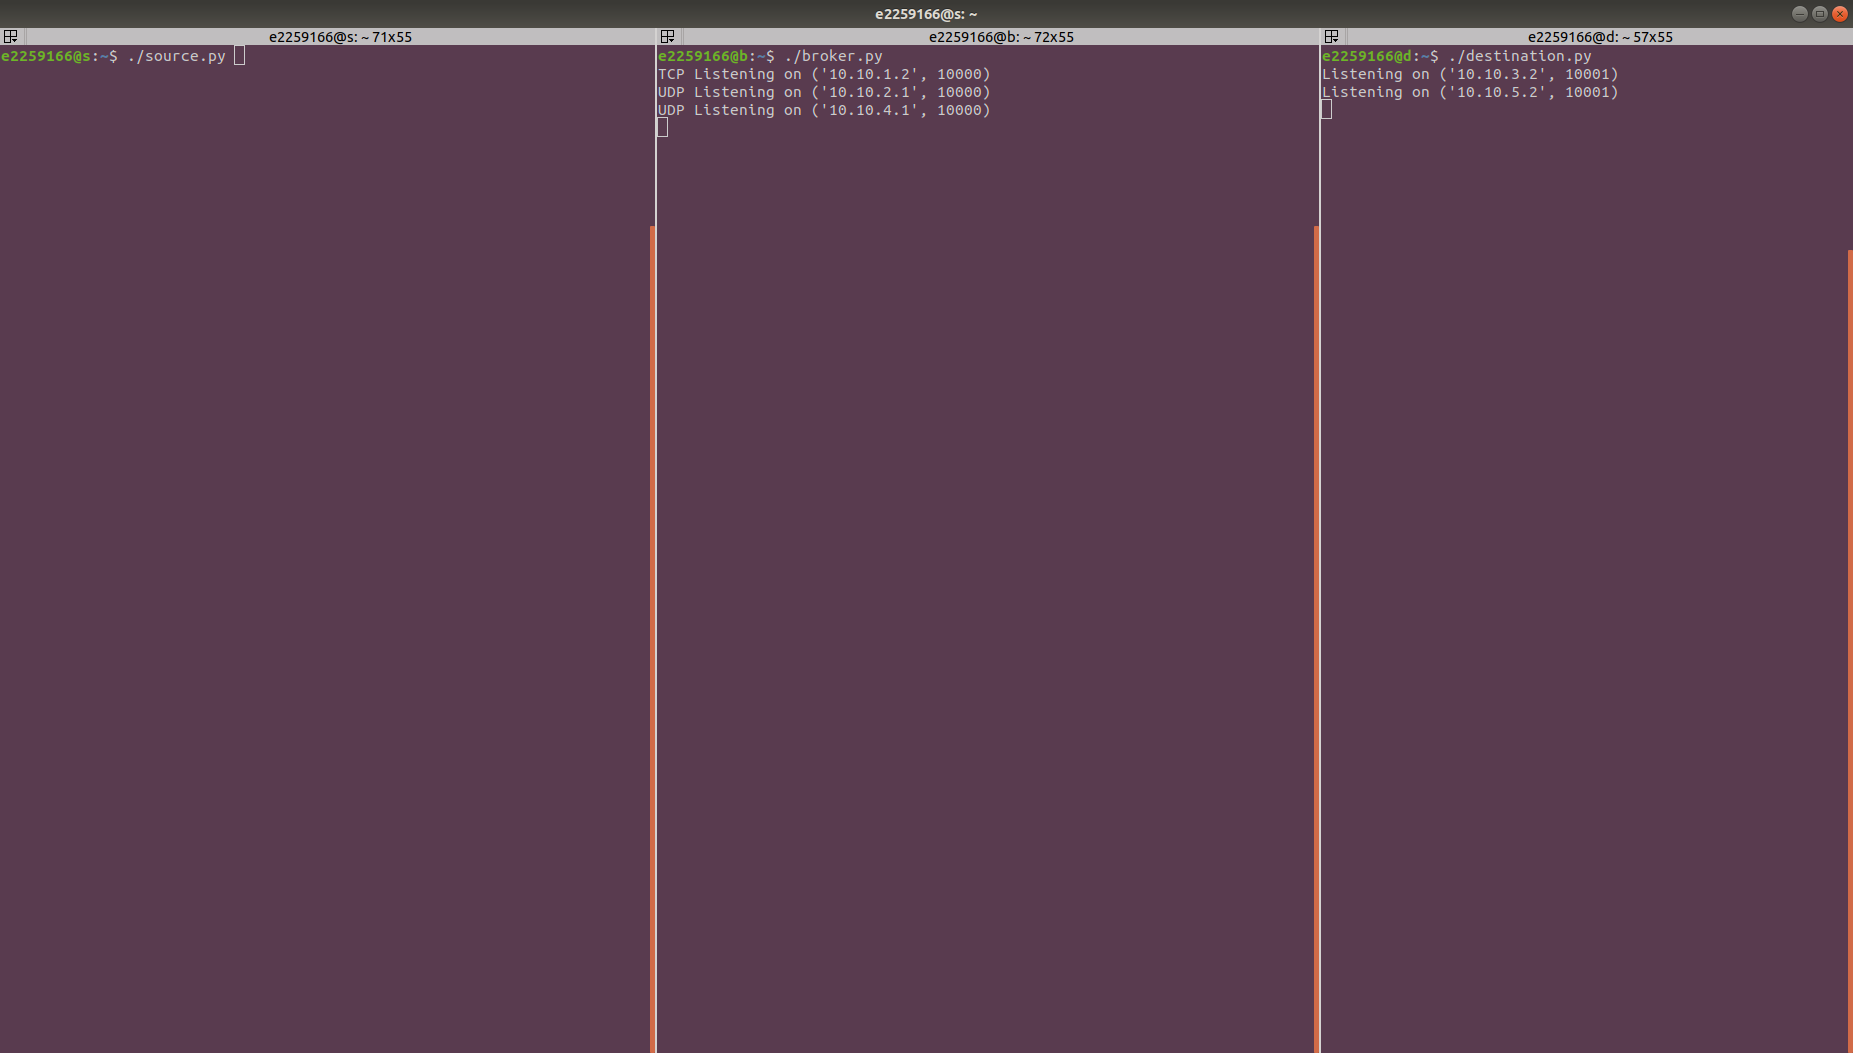
\includegraphics[scale=0.13]{start_up.png}
    \caption{Example start up vision for execution}
\end{figure}

\begin{figure}[H]
    \centering
    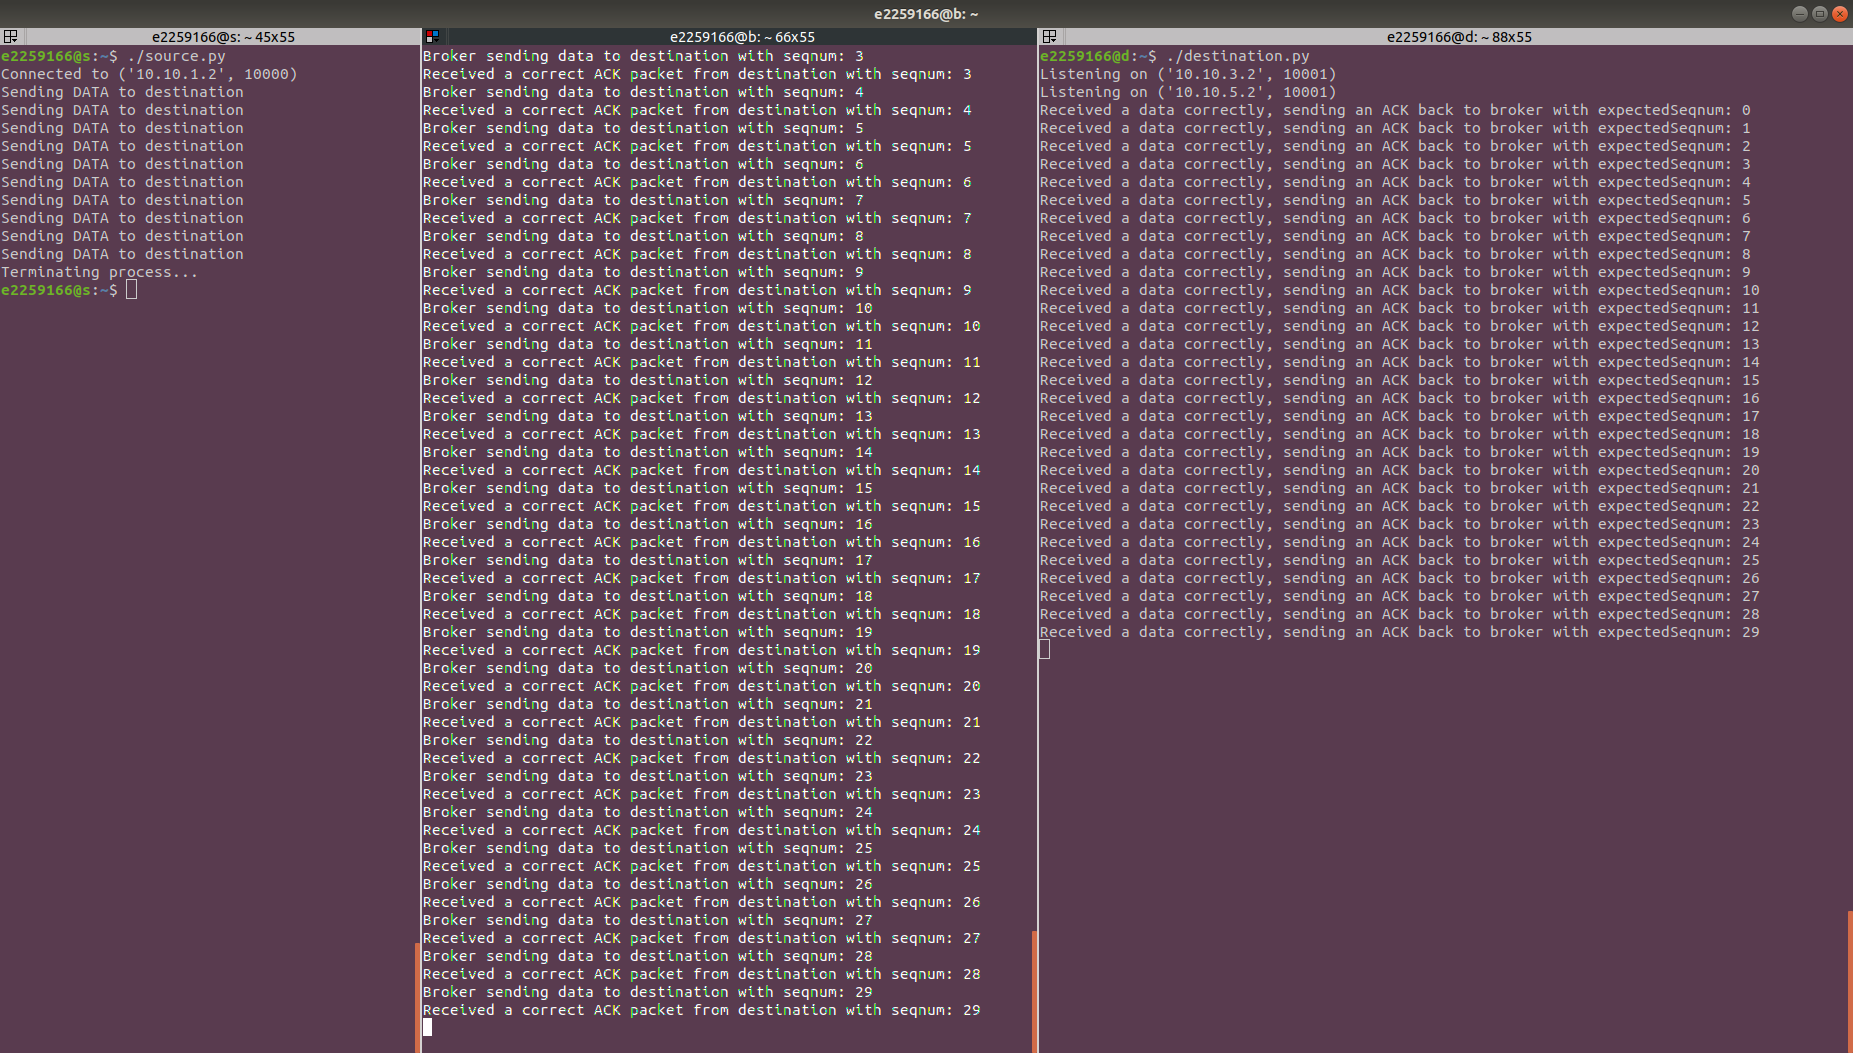
\includegraphics[scale=0.13]{halfway_execution.png}
    \caption{Example halfway execution vision}
\end{figure}

\begin{figure}[H]
    \centering
    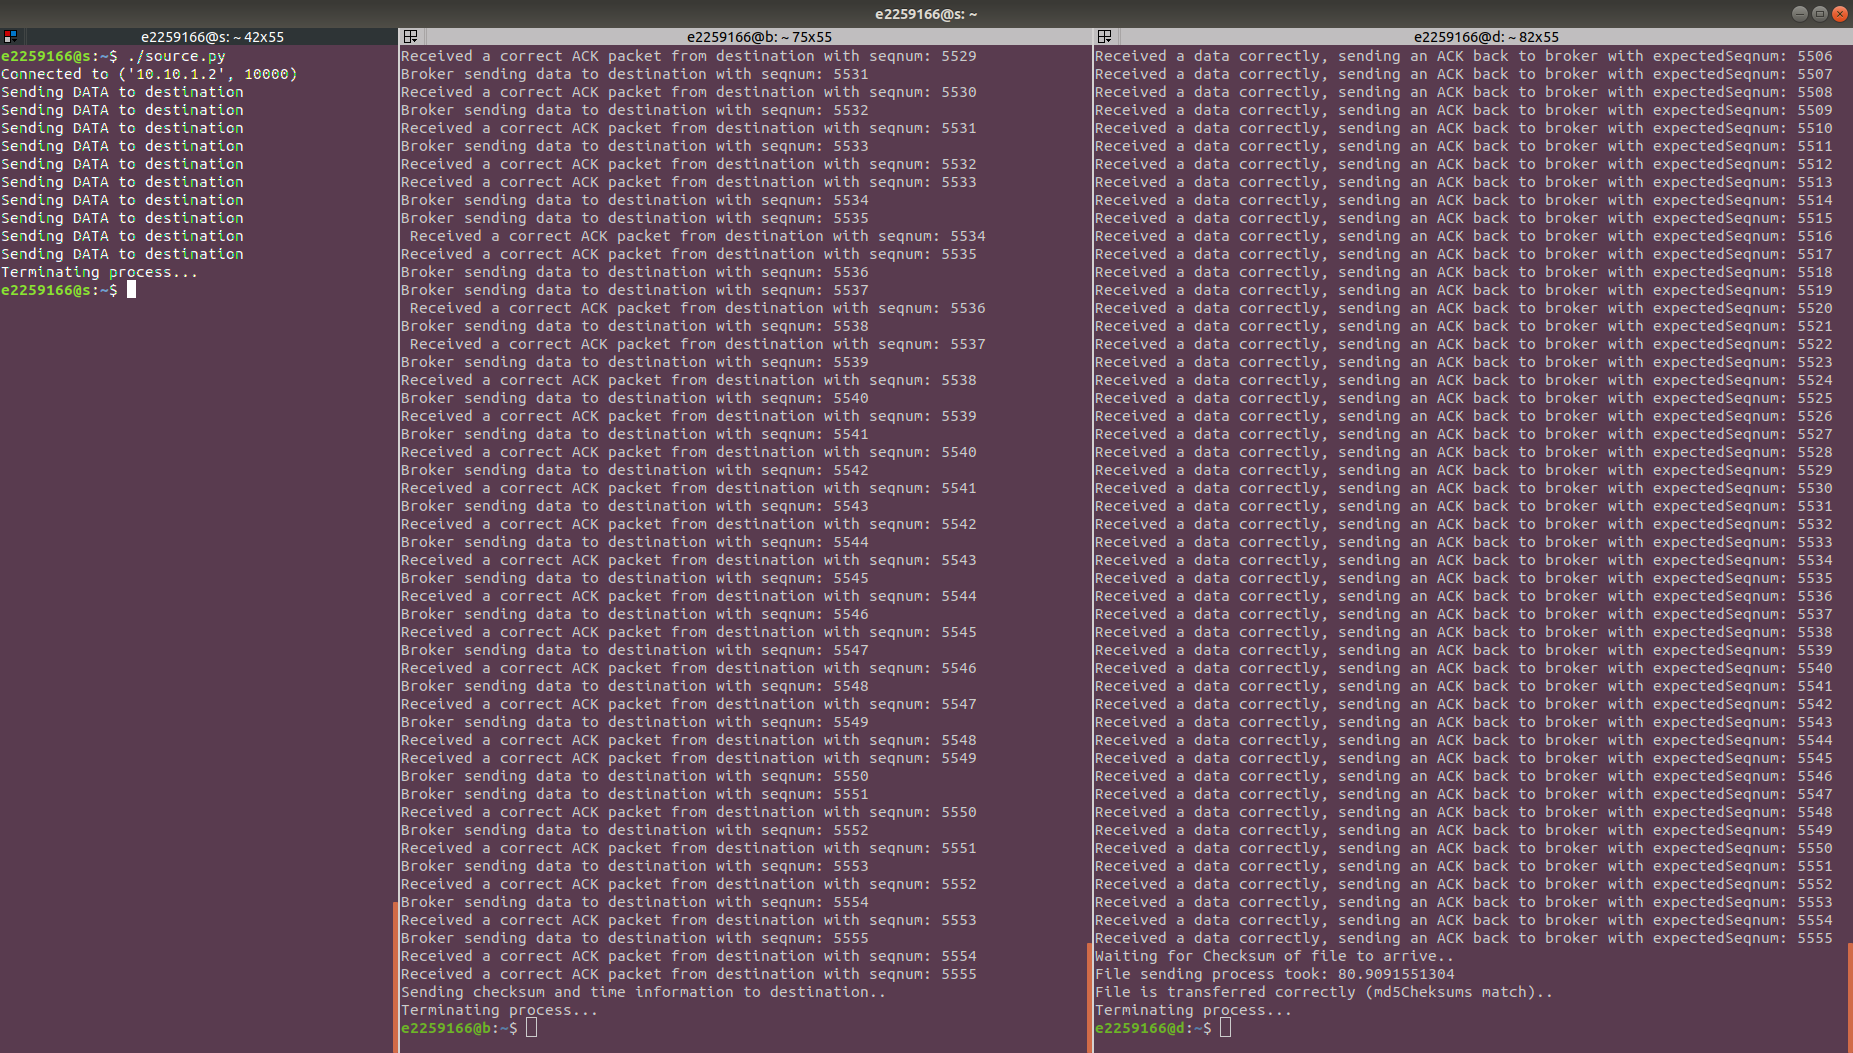
\includegraphics[scale=0.13]{finish.png}
    \caption{Example finish vision}
\end{figure}

\section{Methodology and Motivation}
\subsection{Methodology}
By using "struct" and "time" libraries of Python, time information is added into packets to calculate end to end delay. \\
"threading" and "socket" libraries of Python are used to implement TCP and UDP at the application level and to create multithreaded structure. Also "hashlib" library is used for generating checksum (md5sums) of the data whenever needed.

\subsection{Motivation}
This project was helpful for us to learn and experience topics like socket programming with different transport layer protocols, scripting languages and multithreaded structures. We have learned different terms and tools related with stream, packets, protocols and network delay. We have also practiced how to measure or manipulate them.  We have become familiar with the roles of different nodes in networks such as router, broker, receiver and sender nodes. We have learned how to configure routers to forward desired packets from one end to other. We have also learned how to synchronize the computers and how to add, show, delete network emulation delays.\\

In addition, We have learned the fundamental differences between TCP and UDP and how to implement a reliable data transfer protocol on top of an unreliable channel. In this manner, this part of the project was helpful for us to fully understand the fundamental structures of reliability in network and how to provide it in terms of lost, corrupt and change of order in packets with multihoming and pipelining in the network. 

\section{Experimental Results}
\subsection{Tools Used For Experiments}
\textbf{NTP}:
NTP (Network Time Protocol) is a protocol that is used to synchronize clock of computer systems overpacket-switched networks. We used NTP because sending the data computerclock is in nanoseconds, but in network systems packets are sent probably in microseconds, so the packets are received before its time because of the asynchronization. \\

\textbf{Linux Traffic Control}:
Traffic control (tc) is a very useful Linux utility that gives you the ability to configure the kernel packet scheduler. It allows us to utilize Linux’s helpful tools to simulate packet delay and loss for UDP or TCP applications, or limit the bandwidth usage of a particular service to simulate Internet connections (DSL, Cable, T1, etc.) \\

\textbf{Netem}:
NetEm is an enhancement of the Linux traffic control facilities that allow to add delay, packet loss, duplication and more other characteristics to packets outgoing from a selected network interface. In our experiments we used this command for emulating the delay loss and other similar properties of our network. To achieve this, we applied various kinds of this command for each network interface of the nodes and with some parameters for the virtual machines we created in GENI.

\subsection{Experimental Part}
For this part, we mainly made three experiments with three subcases each and plot the information that we gather from these experiments. Since we were needed to repeat the experiment for a considerable amount of time to get meaningful results, we repeated execution exactly 36 times for each experiment. We sent a file of size 5MB(megabytes) from source node to destination 36 times for each case, and collected necessary results. \\

The commands that we used for delete, show and add for each experiment are indicated on the README file. \\

Main task was to calculate file transfer time from source to destination node, and as mentioned earlier on this report, to achieve this, destination node was calculating time passed since source node started to send the file. Since we execute our sending data from source to destination process $36$ times; we had to measure every case 36 times and store the results we get, then calculate the statistics of our experiment. \\

Following figures (Figure 4,5,6) show example executions of an experiment for each figure. 

\begin{figure}[H]
    \centering
    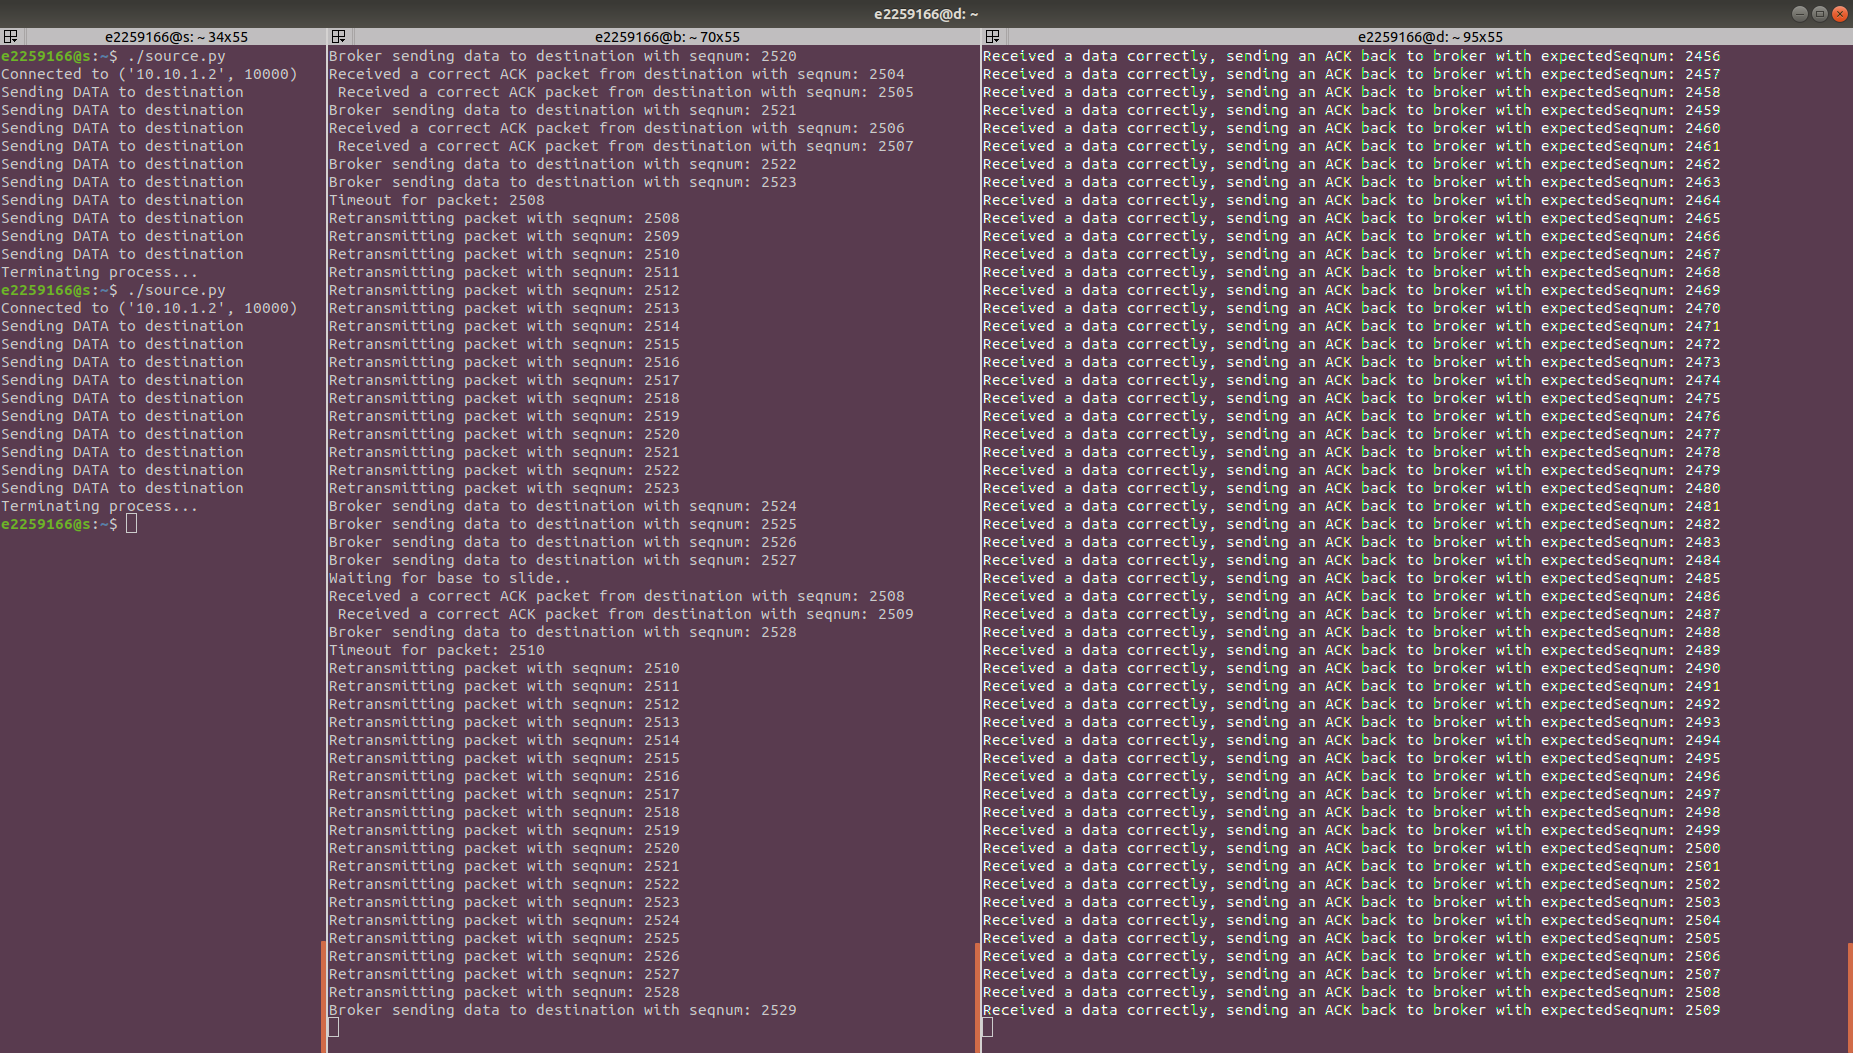
\includegraphics[scale=0.13]{fig1.png}
    \caption{Example execution of 1st experiment in 1st figure}
\end{figure}

\begin{figure}[H]
    \centering
    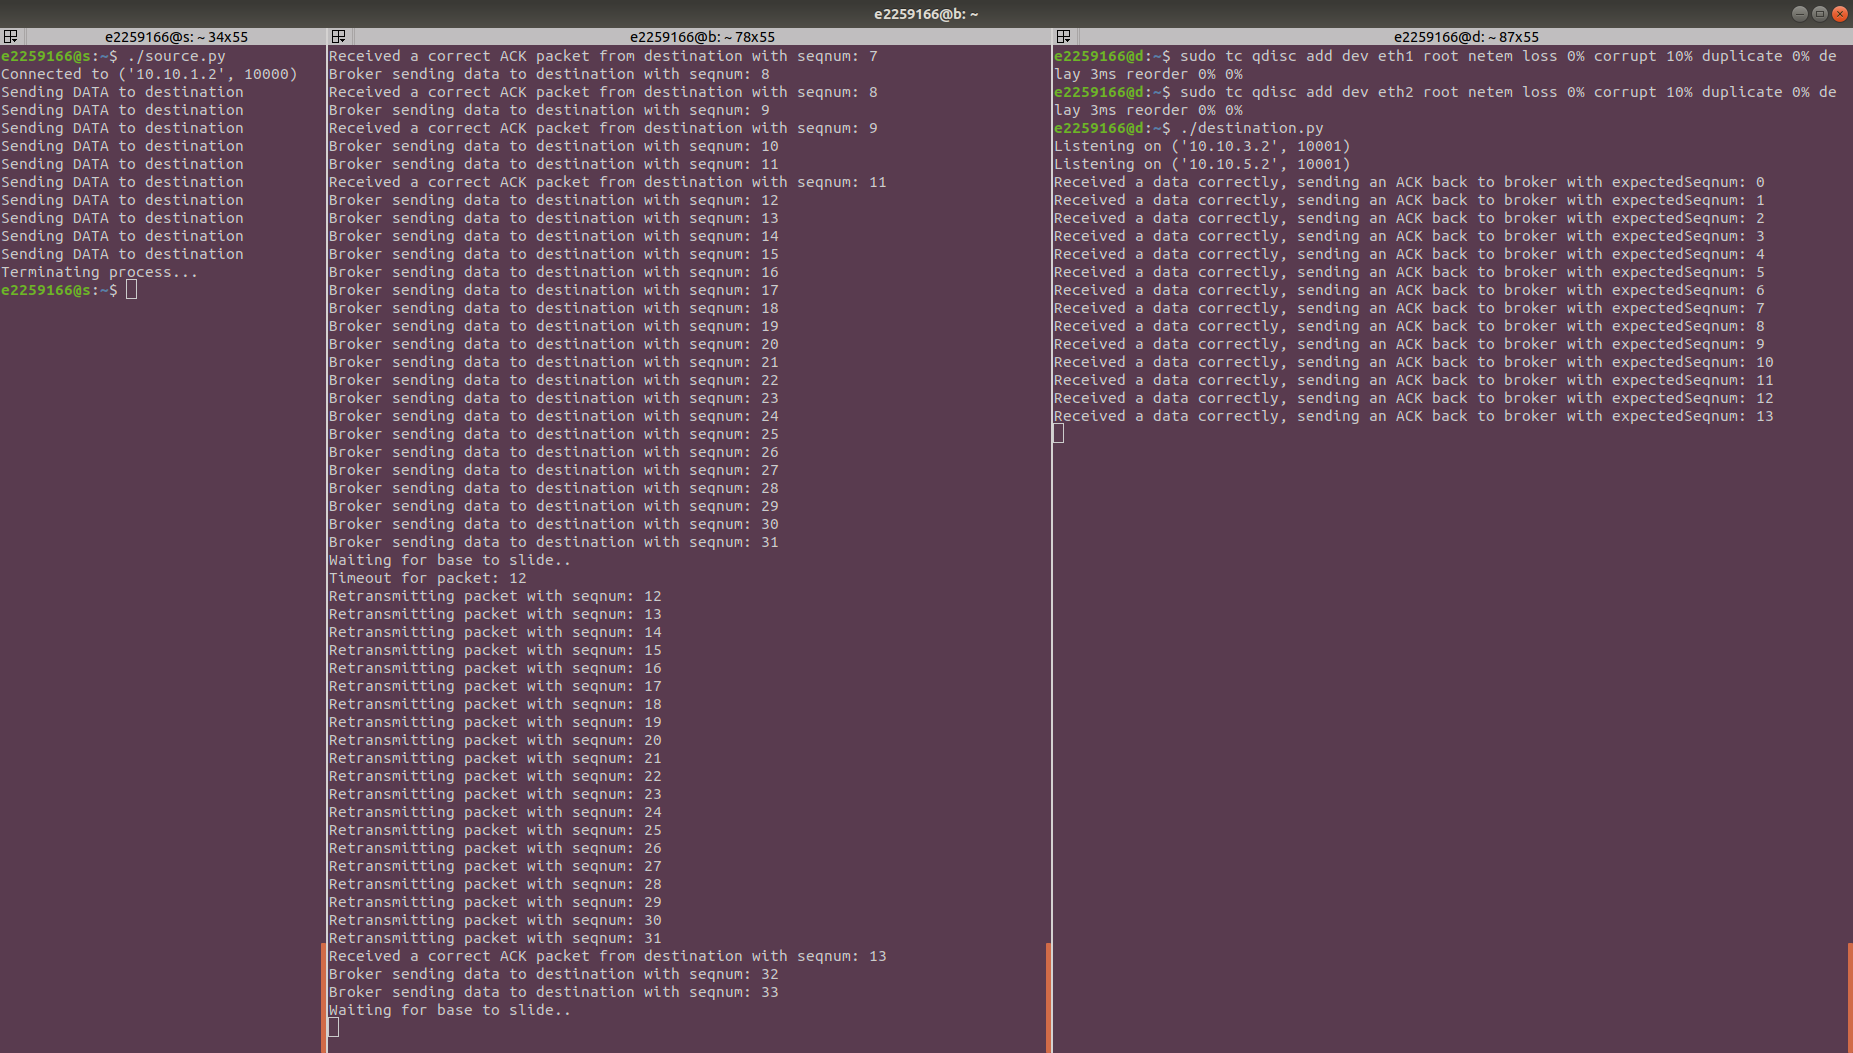
\includegraphics[scale=0.13]{fig2.png}
    \caption{Example execution of 2nd experiment in 2nd figure}
\end{figure}

\begin{figure}[H]
    \centering
    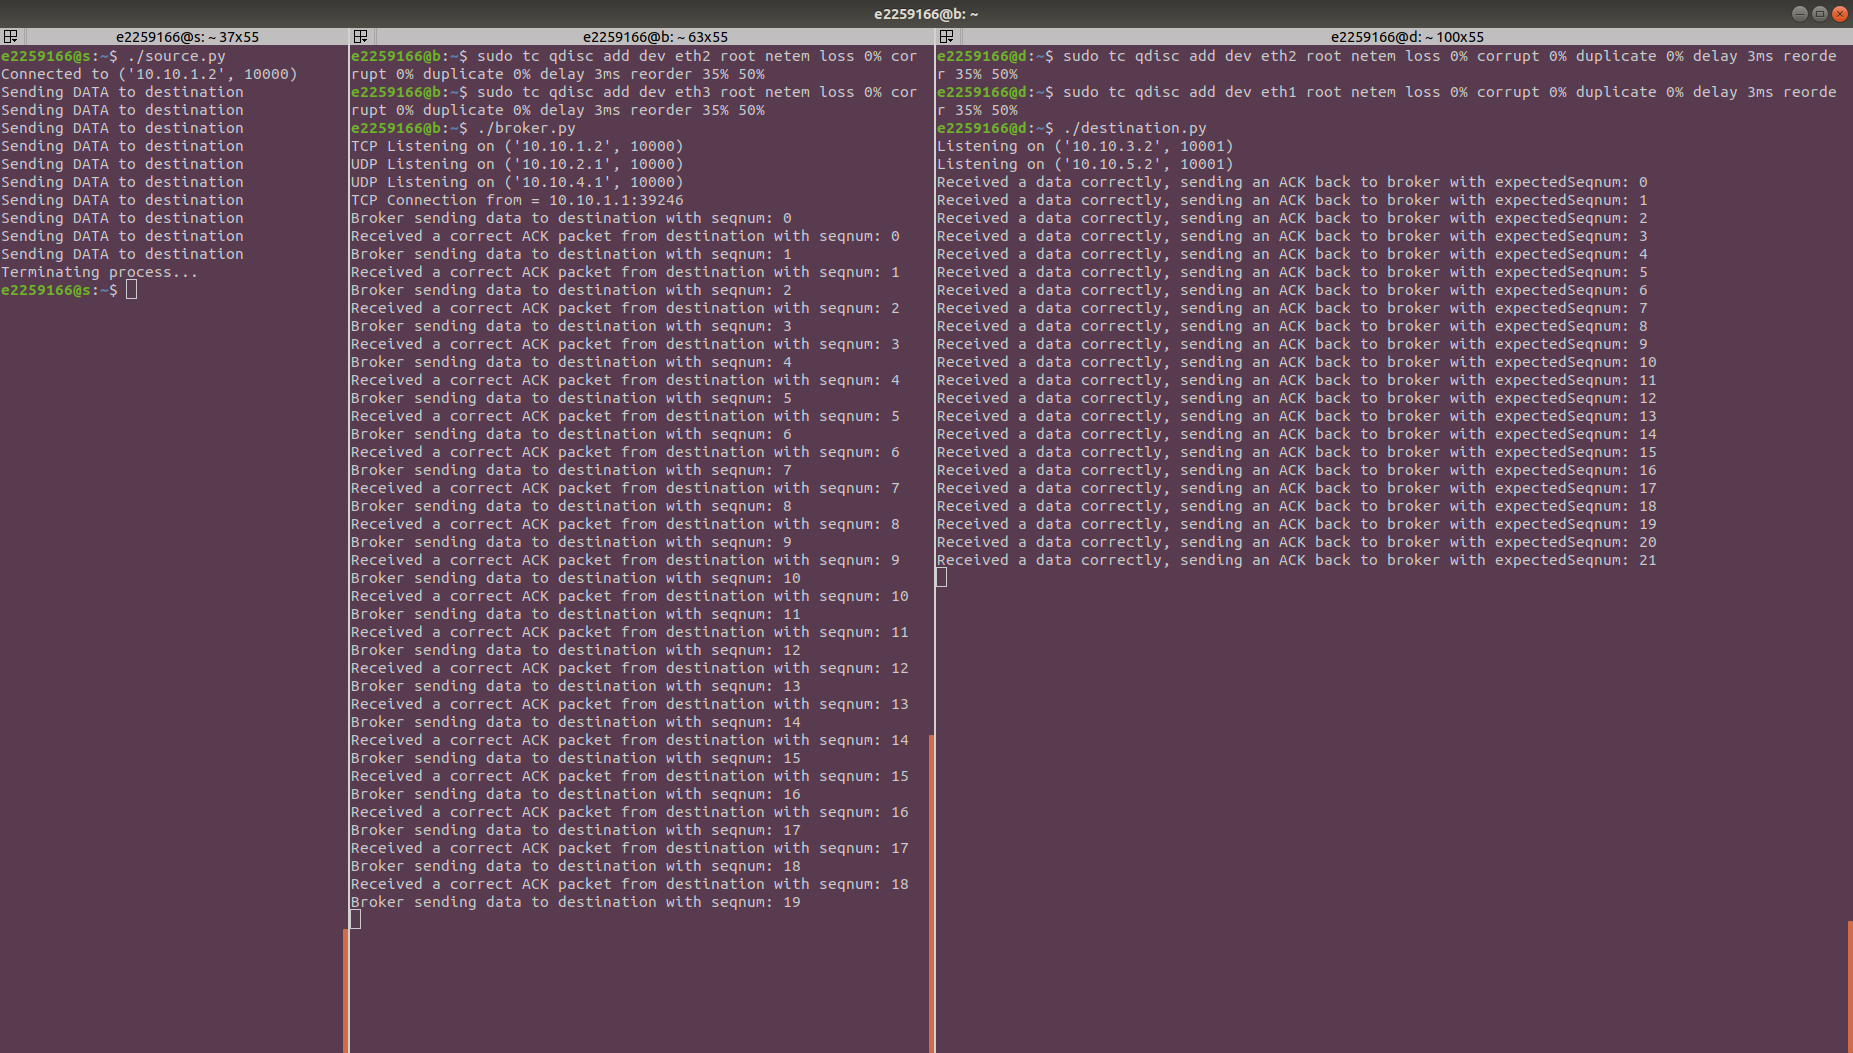
\includegraphics[scale=0.13]{fig3.png}
    \caption{Example execution of 3rd experiment in 3rd figure}
\end{figure}

For each experiment we calculated sample mean(m), sample standard deviation(e) and error of the experiment(e). In order to find margin of error for the experiment we used the following formula. \\
\begin{align*}
 e &= z \times \frac{(\text{standard deviation for that experiment's delays})}{\sqrt{\text{number of executions}}}  \\\\
   &= 1.960 \times \frac{(\text{standard deviation for that experiment's delays})}{\sqrt{36}} \\
\end{align*}
Where $z$ is the confidence interval variable (for our case, confidence interval = 95\% , so z = 1.960). 

\begin{figure}[h]
    \centering
    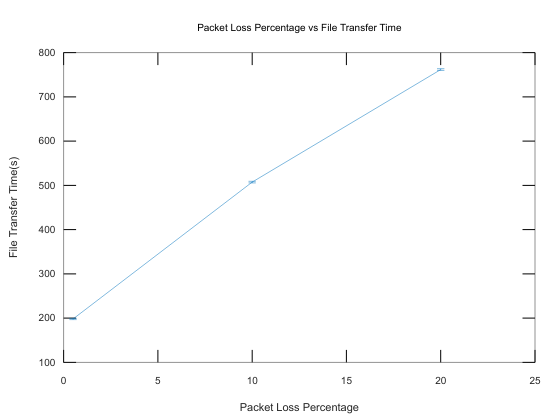
\includegraphics[scale=0.45]{graph1.png}
    \caption{Packet Loss Percentage vs File Transfer Time}
\end{figure}

For the first experiment, we executed our process on a network with $0.5\%,10\%,20\% $ packet loss respectively, also with an 3ms additional delay. Afterwards, we executed it $36$ times for each percentage of packet loss. Figure 7 is the graph we plot using statistic of our three cases. x-axis denotes the packet loss percentages and the y-axis shows the corresponding file transfer time in seconds. The sample mean value we calculated for three cases were $(198.1 , 507.4 , 761.6)$ seconds respectively. Standart deviations were $4.097, 5.250, 5.898$ again respectively. Knowing standart deviations we calculated margin of errors as $e=(1.338 , 1.715 , 1.926)$ which for all cases smaller than 2.5 thus, appropriate for experiment. The error of margin is denoted over the line of the graph with 2 horizontal small lines meaning the value may change inbetween these small lines. One thing we can observe from this figure is the transfer time increases with the percentage of loss packets. It makes sense since when a lost packet occurs, the source node sends the packet again and again until it arrives the destination and source node acknowledges that, which returns as a delay in transfer. The increase on delay that comes with loss packet percentage is in a linear fashion as it can be observed from the graph. Also note that we added these loss packet percentages to all links between broker and destination nodes(meaning exactly 2 links for both interfaces). If we were to apply lost packets in only 1 link, we would get different results.  


\begin{figure}[h]
    \centering
    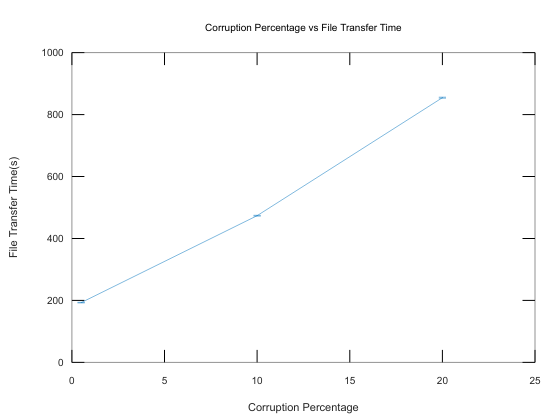
\includegraphics[scale=0.45]{graph2.png}
    \caption{Corruption Percentage vs File Transfer Time}
\end{figure}

On the second part of experiment, we executed our process on a network with $0.2\%,10\%,20\% $ corruption rate and 3ms of additional delay. Afterwards, we executed it $36$ times for each case of corruption rates. Figure 8 is the graph we plot using statistic of our three cases. x-axis stands for corruption rates and the y-axis denotes the corresponding file transfer time in seconds. The calculated sample mean value for three cases were $(193.1 , 473.5 , 854.4)$ seconds respectively. Standart deviations were $2,755, 3,804, 4.974$ again respectively. This information allowed us to calculate margin of errors as $e=(0.900 , 1.242 , 1.625)$ which for all cases smaller than 2.5 means it is appropriate for experiment. The error of margin is denoted over the line of the graph with 2 horizontal small lines meaning the value may change inbetween these small lines. One thing we can observe from this figure is the transfer time increases with the percentage of loss packets. It is logical since a packet corrupts, destination node will understand that it is corrupt thanks to checksum, and the source node sends the packet again and again until the packet arrives the destination without a corruption, which returns as a delay in transfer. The increase on delay that comes with loss packet percentage is in a linear fashion as the graph seems like line. Also note that we added these corruption rate to all links between broker and destination nodes(meaning exactly 2 links for both interfaces). If we were to apply lost packets in only 1 link, we would get different results.  


\begin{figure}[h]
    \centering
    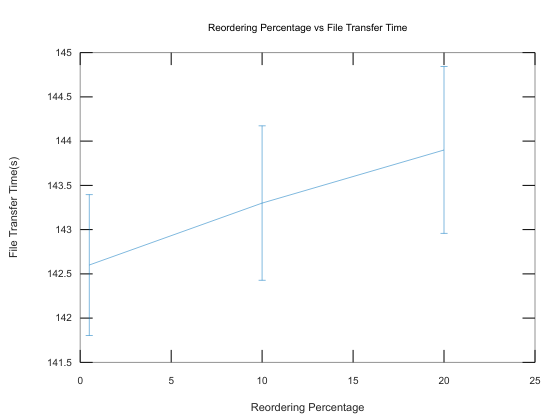
\includegraphics[scale=0.45]{graph3.png}
    \caption{Reorder Rate vs File Transfer Time}
\end{figure}

On the third and last experiment, we executed our process on a network with $1\%,10\%,35\% $ reorder rate and 3ms of additional delay. Then, we executed it $36$ times for each case of reorder rates. Figure 9 is the graph we plot using statistic of our three cases. x-axis stands for reorder rates and the y-axis shows the corresponding file transfer time in seconds. The calculated sample mean value for three cases were $(142.6 , 143.3 , 143.6)$ seconds respectively. Standart deviations were $2,437, 2,670, 2,886$ again respectively. Then we calculated margin of errors as $e=(0.796 , 0.872 , 0.942)$ which for all cases smaller than 2.5 means it is appropriate for experiment. The error of margin is denoted over the line of the graph with horizontal lines meaning the value may change inbetween these lines. Note that y values of graph are between 141.5 and 145 so the y axis of graph is zoomed in. One thing we can observe from this figure is the transfer time does not increase significantly with the reorder rate, only a small amount of increase happens. It is not like corrupt or lost packets because reordered packets does not require source to resend said packets because destination keeps the not-in-order packets in The increase on delay that comes with loss packet percentage is in a linear fashion as the graph seems like line. We add these corruption rate to all nodes inbetween broker and destination nodes, if we were to apply lost packets to only one device, we would get different results. Also note that we added these reordering rate to all links between broker and destination nodes(meaning exactly 2 links for both interfaces). If we were to apply lost packets in only 1 link, we would get different results.  

\end{document}
